\documentclass[review]{elsarticle}

\usepackage{hyperref}
%\usepackage{lineno,hyperref}
%\modulolinenumbers[5]

\journal{European Journal of Operational Research}

%%%%%%%%%%%%%%%%%%%%%%%
%% Elsevier bibliography styles
%%%%%%%%%%%%%%%%%%%%%%%
%% To change the style, put a % in front of the second line of the current style and
%% remove the % from the second line of the style you would like to use.
%%%%%%%%%%%%%%%%%%%%%%%

%% Numbered
%\bibliographystyle{model1-num-names}

%% Numbered without titles
%\bibliographystyle{model1a-num-names}

%% Harvard
%\bibliographystyle{model2-names.bst}\biboptions{authoryear}

%% Vancouver numbered
%\usepackage{numcompress}\bibliographystyle{model3-num-names}

%% Vancouver name/year
%\usepackage{numcompress}\bibliographystyle{model4-names}\biboptions{authoryear}

%% APA style
\bibliographystyle{model5-names}\biboptions{authoryear}

%% AMA style
%\usepackage{numcompress}\bibliographystyle{model6-num-names}

%% `Elsevier LaTeX' style
%\bibliographystyle{elsarticle-num}
%%%%%%%%%%%%%%%%%%%%%%%

%My Packages
\usepackage{amsmath,amsfonts,amssymb,amsthm}
\usepackage{thmtools}

\declaretheoremstyle[bodyfont=\normalfont,]{defn}
    \newcommand{\sub}[1]{_{\text{#1}}} %für Indizes in normaler Schrift unten
    \newcommand{\up}[1]{^{\text{#1}}} %für Indizes in normaler Schrift oben
    \newtheorem{thm}{Theorem} %[section]
    \newtheorem{lem}[thm]{Lemma}
    \newtheorem{cor}[thm]{Corollary}
    \newtheorem{prop}[thm]{Proposition}
    \theoremstyle{defn}
    \newtheorem{defn}[thm]{Definition}    
    \newtheorem{rem}[thm]{Remark}  

    \newtheoremstyle{Pseudo-Code}% name of the style to be used
      {\topsep}% measure of space to leave above the theorem. E.g.: 3pt
      {\topsep}% measure of space to leave below the theorem. E.g.: 3pt
      {}% name of font to use in the body of the theorem
      {0pt}% measure of space to indent
      {\bfseries}% name of head font
      {\noindent}% punctuation between head und body
      {\newline}% space after theorem head; " " = normal interword space
      {}% Manually specify head
    \theoremstyle{Pseudo-Code}
    \newtheorem{Pseudo-Code}{Algorithm}

%IstlistingAnfang*******************************************
\usepackage{color}
\usepackage{listings}

\lstdefinelanguage{Pseudo-Code}{morekeywords={And, Algorithmus, Alg, As, Byte, ByRef, Call, Case, Cells, Compare, Count, Date, Dim, Do, Double, Else, ElseIf, End, Error, Exit, Explicit, False, For, Function, GoTo, If, Integer, Loop, MInverse,  MMult, Next, Not, Nothing, Object, On, Option, Or, Private, Return, Resume, Row, Rows, String, Single, Select, Set, Sub, Then, , Transpose, True, To, UBound, Variant, While, WorksheetFunction, Print,}, 
    sensitive=false, 
%    morecomment=[l]Rem, 
    morecomment=[l]', 
%    morestring=[b]", 
%    emph={MsgBox,}, 
%    emphstyle=\itshape
} 

\lstdefinestyle{Pseudo-Code}
{
    framesep=0pt,%expand outward.
    framerule=0pt,%expand outward.
    xleftmargin=0pt,%make the frame fits in the text area. 
    xrightmargin=0pt,%make the frame fits in the text area.    
    %backgroundcolor=\color{Black},
    basicstyle=\normalsize\color{black},
    keywordstyle=\ttfamily,
    identifierstyle=\slshape,
    %stringstyle=\color{Red},
    %commentstyle=\color{green},
    language={Pseudo-Code},
    tabsize=2,
    %numbers=left,
    %fontadjust=true,
    %keepspaces=true,
    %showspaces=true
    columns=flexible,
    escapechar={§}
}

\lstset{literate=%
  {Ö}{{\textsl{\"O}}}1
  {Ä}{{\textsl{\"A}}}1
  {Ü}{{\textsl{\"U}}}1
  {ß}{{\textsl{\ss}}}2
  {ü}{{\textsl{\"u}}}1
  {ä}{{\textsl{\"a}}}1
  {ö}{{\textsl{\"o}}}1
}
%IstlistingEnde*******************************************

 \usepackage{pgfplots}
    \usepackage{pgfplotstable}
  \pgfplotsset{compat=1.13}


 %Einheiten
  \usepackage[binary-units=true]{siunitx} 

\begin{document}

\begin{frontmatter}

\title{Computation of the Johnston Power Index in Weighted Majority Games}
%\tnoteref{mytitlenote}}
%\tnotetext[mytitlenote]{Fully documented templates are available in the elsarticle package on \href{http://www.ctan.org/tex-archive/macros/latex/contrib/elsarticle}{CTAN}.}

%% Group authors per affiliation:
%\author{Elsevier\fnref{myfootnote}}
\author{Ingo Wilms\fnref{myfootnote}}
%\address{Habichtshofring 25, 22175 Hamburg, Germany}
\fntext[myfootnote]{ingo.wilms@gmail.com}

%% or include affiliations in footnotes:
%\author[mymainaddress,mysecondaryaddress]{Ingo Wilms}
%\author[mymainaddress]{Ingo Wilms}
%\ead[url]{www.elsevier.com}

%\author[mysecondaryaddress]{Global Customer Service\corref{mycorrespondingauthor}}
%\cortext[mycorrespondingauthor]{ingo@imazeki.de}
%\ead{support@elsevier.com}

%\address[mymainaddress]{Habichtshofring 25, 22175 Hamburg, Germany}
%\address[mysecondaryaddress]{}

\begin{abstract}
Power indices can be very useful to reveal the actual power of voters in a voting system. In weighted majority games each voter has a weight and the overall vote is ``yes'', if the sum of weights of all ``yes''-voters is greater or equal the quota.
One of the power indices that is regularly the subject of research is the Johnston index.
In this paper I propose an algorithm for the computation of the Johnston power index in weighted majority games.
The presented algorithm computes the index in pseudo-polynomial time, if the single weights are all integers. 
% \PACS{PACS code1 \and PACS code2 \and more}
% \subclass{MSC code1 \and MSC code2 \and more}
\end{abstract}

\begin{keyword}
Game theory \sep Power indices \sep Johnston index \sep Generating functions \sep Weighted majority games
\end{keyword}

\end{frontmatter}

%\linenumbers


\section{Introduction}
\label{intro}
Power indices can be used to describe the power of players in a voting system. Each player votes ``yes'' or ``no'' over a proposal. All ``yes''-voters form a coalition and all ``no''-voters form a coalition. According to predefined rules it is determined, which coalition is winning. 
Although the concept of power is somewhat abstract, in the domain of power indices a voter usually is said to have power, if the voter can influence the outcome with his vote \citep{Penrose1946}.
 In weighted majority games each player has a voting weight and a coalition is considered winning if the sum of the weights of all members in that coalition is equal or bigger than a certain quota $q$.

Several power indices were suggested in the past. Two of the best researched and most often applied power indices are Banzhaf index \citep{Penrose1946, Banzhaf1965} and Shapley-Shubik index \citep{Shapley1954}.
The Deegan-Packel index \citep{Deegan1978} and the Johnston index \citep{Johnston1978} played a minor up to today. 
On the one hand the Johnston index has been criticized for some of its properties by \cite{FelsenthalMachover1998}, but on the other hand \cite{Brams1990} advocated the index especially for the measurement of presidential power.  \cite{Brams1990} applied the Johnston index to the United States federal system and \cite{Mercik2009} applied the index to the polish president.

Although the Johnston index is regularly the subject of theoretical research (for instance \cite{Hirokawa2006}, \cite{Alonso-Meijide2007}, \cite{Alonso-Meijide2008}, \cite{Freixas2012}, \cite{Freixas2013} and \cite{Kurz2016}), except for \cite{Alonso-Meijide2008} no effort has been made to establish computational methods.
\cite{Alonso-Meijide2008} describe an algorithm for the computation of the Johnston index using the multilinear extension method introduced by \cite{Owen1972}. In general this method has its strength in approximating power indices for large number of players $n$ as the exact computation has exponential time complexity.  %\citep{Leech2002b}.

Due to lack of exact computational methods even for moderate $n$ it is not surprising there are only very few cases in the literature, where the Johnston index was applied to real world weighted majority games. Two examples are \cite{Strand2003} and \cite{Strand2005}. In both cases the authors used an own program combining an enumeration method and the generating functions technique.
%An efficient algorithm for the calculation of Banzhaf index, Shapley-Shubik index and Deegan-Packel index \citep{Deegan1978} was proposed by \cite{Matsui2000} and later improved by \cite{Uno2003}. Therefore it is not surprising that an efficient algorithm for the Johnston index exists.

%\cite{Alonso-Meijide2007}.
%\cite{Laver1978} critisized Johnston for using the normalized version of the Banzhaf index. He argued the more decisive players there are the more fragile a coalition becomes. That would lead to less power for each decisive player. In response to that argument Johnston suggested - instead of assigning a value of 1 to each decisive player of every winning coalition as the Banzhaf index does - to assign an overall value of 1 for each winning coalition that has to be shared equally among the decisive players. 
%The assigned values can also be seen as a payoff.
%Consider a payoff of one for each winning coalition that has to be shared equally among all decisive players.
%The Johnston index of one player can then be interpreted as her/his expected share of the overall payoff of all players if every coalition is equally probable.
% As there is no consensus about what is the best power index to use it seems surprising that except for small examples practical applications of the Johnston index cannot be found in the literature. 
% A reason for this could be the lack of computational methods. Without any efficient algorithms the computation of the Johnston index can be expensive, as a naive implementation will take $\mathcal{O}(n2^n)$ time, where $n$ is the number of players.
% 
With this article I want to propose a new algorithm for the exact computation of the Johnston index in weighted majority games.
For the calculation of Banzhaf index, Shapley-Shubik index and Deegan-Packel index for all $n$ players there exist algorithms with time complexity $\mathcal{O}(nq)$, $\mathcal{O}(n^2q)$ and $\mathcal{O}(n^2q)$ respectively \citep{Uno2003}.
I will use similar techniques to develop an algorithm for the computation of the Johnston index of all players within time complexity $\mathcal{O}(n^3q)$, which uses $\mathcal{O}(nq)$ memory.


\section{Preliminaries}
Let $N=\{p_1,p_2,\dots,p_n\}$ be a set of players. Every subset $S\subseteq N$ is called a coalition.
Let $w_i\in\mathbb{N}$ be the weight of player $p_i$, $i=1,2,\dots,n$. Then we can define the weight function 
\begin{align*}
  w:\{S\subseteq N\}\rightarrow\mathbb{N}, 
  S\mapsto w(S):=\sum_{p_i\in S} w_i.
\end{align*}
A weighted majority game is represented by $[q;w_1,w_2,\dots,w_n]$ where $q\in\mathbb{N}$ is the quota satisfying $\frac{1}{2}\sum_{i=1}^n w_i<q\leq w(N)$. A coalition $S\subseteq N$ is called winning if and only if $w(S)\geq q$.
The set of all winning coalitions is denoted by $W$.
A player $p_i$ is said to be \emph{crucial} for $S$, if $w(S)\geq q$, $p_i\in S$ and $w(S\setminus \{p_i\})<q$. I will denote the set of all winning coalitions containing at least one crucial player with $W_\text{qmin}$.


\begin{defn}
Let $[q;w_1,w_2,\dots,w_n]$ be a weighted majority game. The Johnston index of player $p_j$ is defined by
\begin{align}
  \label{eqn:Johnston}
  \gamma_j
  &\cdot 
  |W_\text{qmin}|
  =
  \sum_{\substack{S\in W_\text{qmin}:
    \\
     w(S\setminus p_j)<q}}
  \frac{1}{\#\{p_i\in S:w(S\setminus p_i)<q \}}
  .
\end{align}
\end{defn}

\section{Computation of the Johnston Index}

\begin{rem}
Without loss of generality we assume $w_1\geq w_2\geq \cdots \geq w_n$. If the weights are not sorted, they have to be sorted by using a sorting algorithm. The time complexity of well known sorting algorithms is bounded by $\mathcal{O}(n\log n)$.
\end{rem}


We define two subsets of $N$ by
\begin{align*}
  P_i
  &=
  \{p_1,p_2,\dots,p_i\},
\quad\quad
  \overline{P}_i
  =
  \{p_i,p_{i+1},\dots,p_n\}
  .
\end{align*}
Also we define $P_{0}=\overline{P}_{n+1}=\emptyset$.

\paragraph{The idea of the algorithm}
We want to calculate the Johnston index $\gamma_j$ for player $p_j$.
The idea is to partition every winning coalition $S$, where $p_j$ is crucial, into two disjoint subsets. Let $i$ be the biggest index of a crucial player in $S$. We define two subsets of $S$ by
\begin{align*}
  S_1
  &=
  S\cap P_i
\quad 
\text{and}
\quad
  S_2
  =
  S\cap \overline{P}_{i+1}
  .
\end{align*}
It follows $S=S_1\cup S_2$ and $S_1\cap S_2=\emptyset$. Due to sorted weights every player in $S_1$ is crucial while no player of $S_2$ is.
%We can use the identity
%\begin{align*}
%  \{S:S\in W_\text{qmin}, p_j\in S, p_j \text{ is critical}\}
%  &=
%  \bigcup_{i=j}^n \{S_1\cup S_2\},
%\end{align*}
%where
So, for $i=j,j+1,\dots,n$ we pre-calculate the numbers of all possible coalitions  $S_1\subseteq P_i$ with $\{p_i,p_j\}\subseteq S_1$.
Also, for each combination of $i$ and $w(S_1)$ we pre-calculate the numbers of all possible coalitions $S_2\subseteq \overline{P}_{i+1}$ so that following properties hold
\begin{enumerate}
  \item $S=S_1\cup S_2$ is a winning coalition,
  \item $p_i$ is crucial and
  \item no player in $S_2$ is crucial.
\end{enumerate}
Once we have done that, we can calculate $\gamma_j$ from
\begin{align*}
  \gamma_j\cdot |W_\text{qmin}|
  &=
  \sum_{i=j}^n
  \sum_{y=w(\{ p_i,p_j \})}^{q+w_i-1}
  \sum_{k=|\{ p_i,p_j \}|}^i
  \frac{\#\{S_1:|S_1|=k, w(S_1)=y\}
  \cdot
  \#\{S_2\}}{k}
  ,
\end{align*}
where $S_1$ and $S_2$ fulfil the above properties. 
The limits of the sums are chosen according to our requirements.
For counting possible coalitions $S_1$ we will introduce functions $f$ and $f_j$. For counting possible coalitions $S_2$ we will introduce functions $c$, $d$ and $h$. The functions $f$, $c$ and $d$ were already used by \cite{Uno2003}.

I will start with showing how to count the relevant coalitions $S_2$ for given $i$ and $y=w(S_1)$. 
Let $c$
be a function defined by
\begin{align*}  
   c(i,y)
   &=
   \#\{
     S\subseteq \overline{P}_i:
     w(S)=y
   \}.
  \end{align*}
  Then $c(i,y)$ indicates the number of subsets in $\overline{P}_i$ with weight $y$.
 For $i,y$ with $1\leq i\leq n$ and $0\leq y\leq w(N)$ we derive the property
  \begin{align*}
    c(i,y)
    &=
    \#\{
      S\subseteq \overline{P}_i:
      w(S)=y
    \}
\\
    &=
    \#\{
      S\subseteq \overline{P}_i:
      p_i \in S, w(S)=y
    \}    
    +
    \#\{
      S\subseteq \overline{P}_{i+1}:
      w(S)=y
    \} 
\\
    &=
    \#\{
      S\subseteq \overline{P}_{i+1}:
      w(S)=y-w_i
    \}    
    +
    \#\{
      S\subseteq \overline{P}_{i+1}:
      w(S)=y
    \}     
\\
    &=   
    \begin{cases}
      c(i+1,y)+c(i+1,y-w_i) & \text{if } y\geq w_i, \\
      c(i+1,y) & \text{if } y<w_i.
    \end{cases}
  \end{align*}
  With this recursion we can calculate all $c(i,y)$ for $i\in\{1,2,\dots,n+1\}$ and $y\in\{0,1,\dots,\min\{w(\overline{P}_i),q-w_i\}\}$ from the the initial values $c(n+1,0)=1$ and $c(n+1,y)=0$ for $y>0$.
  The time complexity for that is $\mathcal{O}(nq)$.

Let now $d$ be a function defined by
    \begin{align*}
  d(i,z)
  &=
     \begin{cases}
     \#
     \{
       S\subseteq \overline{P}_i:
       w(S)\leq z
     \} & \text{for } z \geq 0, \\
     0 & \text{otherwise.}
   \end{cases}
  \end{align*}
Using the recursion
\begin{align*}
   d(i,z)
   &=
   \sum_{y=0}^z c(i,y)
=
    \sum_{y=0}^{z-1}c(i,y) + c(i,z) 
    =
     d(i,z-1) + c(i,z)
\end{align*}
all values of $d(i,z)$ for $i\in\{1,2,\dots,n+1\}$ and $z\in\{1,2,\dots,\min\{w(\overline{P}_i), q-1\}\}$ can be calculated  in $\mathcal{O}(nq)$.

Now let $h$ be a function defined by
\begin{align*}    
    h(i,y)
    &=
     \#\{
       S\subseteq \overline{P}_{i+1}: 
       y+w(S)-\max\limits_{p_k\in S}w_k \geq q, 
	   y+w(S)-w_i<q
     \}.
  \end{align*}
Then $h$ is exactly the number of $S_2$ for given $i$ and $w(S_1)=y$ that fulfil the properties above.

\begin{prop}
\label{prop:h}
Let $G=[q;w_1,w_2,\dots,w_n]$ be a weighted majority game with $w_1\geq w_2\geq \dots \geq w_n$. Then
\begin{align*}
  h(i,y)
  &=
  \sum\limits_{j=i+1}^{n}
  \Big[
    d(j+1,\min\{q+w_i-w_j-1-y,w(\overline{P}_{j+1})\})
\\
  &\quad
    -d(j+1,\max\{0,q-y\}-1)
  \Big]
  + 
 \begin{cases}
   1 &  \text{if } q+w_i-1\geq y \text{ und } y\geq q \\
   0 & \text{otherwise.}
 \end{cases} 
\end{align*}
\begin{proof}
We write $h(i,y)$ as
\begin{align*}
  h(i,y)
  &=
   \#\{
       S\subseteq \overline{P}_{i+1}: 
       y+w(S)-\max\limits_{p_k\in S}w_k \geq q, 
	   y+w(S)-w_i<q
     \}
\\
  &=
   \#\{
       S\subseteq \overline{P}_{i+1}: 
       y+w(S)-\max\limits_{p_k\in S}w_k \geq q, 
	   y+w(S)-w_i\leq q-1
     \}  
\\
  &=
   \#\{
      S\subseteq \overline{P}_{i+1}: 
       q+w_i-1-y\geq w(S) \geq q-y+\max\limits_{p_k\in S}w_k
     \} 
     .
\end{align*}
Using the identity $\{S\subseteq\overline{P}_{i+1}\}=\bigcup_{j=i+1}^{n+1}\{S\subseteq \overline{P}_{j}: p_j\in S \}$ we obtain
\begin{align*}
  &=
   \#\{\bigcup_{j=i+1}^{n+1}\{
       S\subseteq \overline{P}_{j}: 
       p_j\in S,
       q+w_i-1-y\geq w(S) \geq q-y+w_j
       \}
     \} 
\\
  &=
   \#\{\bigcup_{j=i+1}^{n}\{
       S\subseteq \overline{P}_{j}: 
       p_j\in S,
       q+w_i-1-y\geq w(S) \geq q-y+w_j
       \}  
\\      
 &\quad
 \cup 
  \{S: 
       S=\emptyset,
       q+w_i-1-y\geq 0 \geq q-y
       \}
     \}      
\\
  &=
   \# \{\bigcup_{j=i+1}^{n}\{ 
       S\cup p_j:
       S\subseteq \overline{P}_{j+1}, 
       q+w_i-w_j-1-y\geq w(S) \geq q-y
       \}
\\      
 &\quad    
 \cup 
  \{S: 
       S=\emptyset,
       q+w_i-1-y\geq 0 \geq q-y
       \}
     \}  
     .
\end{align*}
The $\{S:S\subseteq \overline{P}_{j},p_{j}\in S\}$ are pairwise distinct for different $j$. Therefore
\begin{align*}
  &=
  \sum\limits_{j=i+1}^{n}
    \#\{
       S\subseteq \overline{P}_{j+1}: 
         q+w_i-w_j-1-y\geq w(S) \geq q-y
     \}    
\\      
 &\quad   + 
  \#\{S: 
       S=\emptyset,
       q+w_i-1-y\geq 0 \geq q-y
       \}       
       .                                  
\end{align*}
Now substituting $d$ into the equation completes the proof.
\end{proof}  
\end{prop}
This means, after computing $d$ we can compute $h(i,y)$ for $i \in\{1,2,\dots,n\}$ and $y\in \{w_i,w_i+1,\dots,\min\{q + w_i - 1, w(P_i)\}\}$ in $\mathcal{O}(n)$. Therefore, all values of $h(i,y)$ can be computed in $\mathcal{O}(n^2q)$.

I will now address how to count the numbers of $S_1\subseteq P_i$ with $p_i\in S_1$ and $p_j\in S_1$. For that we will use two functions $f$ and $f_j$.
Let
$f$ 
be a function defined by
\begin{align*}
  &f(i,k,y)
\\  
  &=
  \begin{cases}
  \#\{
    S: S\subseteq P_i, w(S)=y, |S|=k\} & \text{for } y\in \{0,1,\dots,w(P_i)\},
  \\
  0 & \text{otherwise.}
  \end{cases}
\end{align*}
$f$ is indicating the number of coalitions in $P_{i}$ for given weight $y$ and number of players $k$.
For $i,k,y$ with $1\leq i\leq n$, $1\leq k\leq i$ and $0\leq y\leq w(P_i)$ we can derive the following property
   \begin{align*}
      f(i,k,y)
      &=
      \#\{
        S: S\subseteq P_i, w(S)=y, |S|=k
      \}
\\
      &=   
      \#\{
        S: S\subseteq P_{i-1}, w(S)=y, |S|=k
      \} 
\\        
      &\quad +
      \#\{
        S: S\subseteq P_{i}, p_i\in S, w(S)=y, |S|=k
      \}         
\\
      &=   
      \#\{
        S: S\subseteq P_{i-1}, w(S)=y, |S|=k
      \}   
\\        
      &\quad +
      \#\{
        S: S\subseteq P_{i-1}, w(S)=y-w_i,|S|=k-1
      \}   
\\
	  &=
    \begin{cases}
      f(i-1,k,y)+f(i-1,k-1,y-w_i) & \text{if } y\geq w_i, \\
      f(i-1,k,y) & \text{if } y<w_i.
    \end{cases}	                    
    \end{align*}
With the initial values
$    f(i,k,0)
    =
    \begin{cases}
      1 & \text{if } k=0 \\
      0 & \text{else.}
    \end{cases}
$
we can calculate $f(i,k,y)$ for all $(i,k,y)\in \{0,1,\dots,n\}\times\{0,1,\dots,i\}\times\{0,1,\dots,q+w_1-1\}$ in $\mathcal{O}(n^2q)$. 


Now let $f_j$ be a function defined by
\begin{align*}
  &f_j(i,k,y)
\\  
  &=
  \begin{cases}
  \#\{
    S:S\subseteq P_{i}\setminus\{ p_j\}, w(S)=y, |S|=k  
  \}
  & \text{for } y\in \{0,1,\dots,w(P_{i}\setminus\{ p_j\})\}, \\
  0 & \text{otherwise.}
  \end{cases}
\end{align*} 
$f_j$ is corresponding to $f(i,k,y)$ setting $w_j=0$.
Completely analogous to before we can show the property
\begin{align*}
  f_j(i,k,y)
  &=
  \begin{cases}
    f_j(i-1,k,y) & \text{for } i=j, \\
    \begin{cases}
    f_j(i-1,k,y) + f_j(i-1,k-1,y-w_i) & \text{if }  y\geq w_i, \\
    f_j(i-1,k,y)                    & \text{if }  y<w_i.
    \end{cases}
    & \text{for }  i\neq j.
  \end{cases}
\end{align*}
Obviously we can calculate $f_j(i,k,y)$ for all $(i,k,y)\in \{0,1,\dots,n\}\times\{0,1,\dots,i\}\times\{0,1,\dots,q+w_1-1\}$ also in $\mathcal{O}(n^2q)$. 


\begin{lem}
\label{lem:pipj}
Let $[q;w_1,w_2,\dots,w_n]$ be a weighted majority game with $i,j\in\{1,2,\dots,n\}$ with $i \geq j$. Then
\begin{align*}
 &\#\{S\subseteq P_i: \{p_i,p_j\}\subseteq S \}
\\ 
 &=
   f(i,k,y)
  -  
   f_j(i,k,y)
  -
  f(i-1,k,y)
  +
  f_j(i-1,k,y)  
  .
\end{align*}
\begin{proof}
Consider the identity
\begin{align*}
  &\{S:S\subseteq P_i\}
\\  
  &=
  \{S:S\subseteq P_i\setminus \{p_i\}\}
  \cup
  \{S:S\subseteq P_i\setminus \{p_j\}\}
  \cup
  \{S:S\subseteq P_i,\{p_i,p_j\}\subseteq S \},  
\end{align*}
or rather the identity of the cardinalities
\begin{align*}
  &|\{S:S\subseteq P_i\}|
\\  
  &=
  |\{S:S\subseteq P_i\setminus \{p_i\}\}|
  +
  |\{S:S\subseteq P_i\setminus \{p_j\}\}|
  -
  |\{S:S\subseteq P_i\setminus \{p_i,p_j\}\}|  
\\  
  &\quad   
  + 
  |\{S:S\subseteq P_i,\{p_i,p_j\}\subseteq S \} |
  .
\end{align*}
If we restrict all sets $S$ to $|S|=k, w(S)=y$ we have
\begin{align*}
 &|\{S:S\subseteq P_i, \{p_i,p_j\}\subseteq S, |S|=k, w(S)=y \} |
\\ 
  &=
  |\{S:S\subseteq P_i, |S|=k, w(S)=y\}|
\\  
  &\quad 
  +
  |\{S:S\subseteq P_i\setminus \{p_i,p_j\}, |S|=k, w(S)=y\}|
\\  
  &\quad 
  -
  |\{S:S\subseteq P_i\setminus \{p_i\}, |S|=k, w(S)=y\}|
\\  
  &\quad   
  -
  |\{S:S\subseteq P_i\setminus \{p_j\}, |S|=k, w(S)=y\}|  
\\
  &= 
  f(i,k,y)
  +
  f_j(i-1,k,y) 
  -
  f(i-1,k,y)
  -  
  f_j(i,k,y)
.
\qedhere
\end{align*}
\end{proof}

\end{lem}


\begin{thm}
\label{thm:Johnston_gamma_j}
Let $[q;w_1,w_2,\dots,w_n]$ be a weighted majority game with $w_1\geq w_2\geq\dots\geq w_n]$. Then
\begin{align*}
  \gamma_j
  &=
  \sum_{i=j}^n
  \sum_{y=w(\{ p_i,p_j \})}^{q+w_i-1}
  \sum_{k=|\{ p_i,p_j \}|}^i
  \scriptstyle
    \left[
      f(i,k,y)-f_j(i,k,y)
      -f(i-1,k,y)+f_j(i-1,k,y)
    \right]
    \frac{1}{k}
    h(i,y)
    .
\end{align*}

\begin{proof}
We rewrite the definition of the Johnston index for player $p_j$ 
\begin{align*}
  &\gamma_j\cdot \#\{ S\subseteq N: w(S)\geq q, \exists p_k\in S: w(S\setminus p_k)<q \}
\\  
  &=
  \sum_{S\subseteq N: w(S)\geq q, p_j\in S, w(S\setminus p_j)<q}
  \frac{1}{\#\{p_k\in S:w(S\setminus p_k)<q \}}
  .
\end{align*}
Partitioning $S=S_1\cup S_2$ as described before leads to
\begin{align*} 
  &=
  \sum_{i=j}^n
  \sum_{\substack{
  (S_1,S_2): 
  \\
  S_1\subseteq P_i: \{p_i, p_j\}\subseteq S_1,
  \\
  S_2\subseteq \overline{P}_{i+1}: p_k\in S_2\Rightarrow w(S\setminus p_{k})\geq q,
\\q+w_i-1\geq
w(S_1\cup S_2)\geq q  
  }}
  \frac{1}{|S_1|}
\\
  &=
  %\scriptstyle
  \sum_{i=j}^n
  \sum\limits_{
    \substack{
      S_1\subseteq P_i: \{p_i, p_j\}\subseteq S_1, 
      \\
      q+ w_i-1 \geq w(S_1)\geq w(\{p_i,p_j\})  }}
    \frac{1}{|S_1|}
   %\scriptstyle
    \#
    \left\lbrace
    \substack{
         S_2\subseteq \overline{P}_{i+1}: 
         \\
         q+w_i-1\geq w(S_1)+w(S_2)\geq q,
         \\
          p_k\in S_2\Rightarrow w(S_1)+w(S_2)-w_k\geq q    
    }
    \right\rbrace  
    .
\end{align*}
Introducing weight $y=w(S_1)$ we can write
\begin{align*}
  &=
  %\scriptstyle
  \sum_{i=j}^n
  \sum_{y=w(\{ p_i,p_j \})}^{q+w_i-1}
  \sum_{
    \substack{
      S_1\subseteq P_i: 
      \\
      \{p_i, p_j\}\subseteq S_1, 
      \\
      w(S_1)=y 
    }
  }
    \frac{1}{|S_1|}
    \#
    \left\lbrace
    \substack{
         S_2\subseteq \overline{P}_{i+1}: 
         \\
         q+w_i-1\geq y+ w(S_2)\geq y+w(S_2)-w_k\geq q\, \forall p_k\in S_2 
     }    
    \right\rbrace
\end{align*}
and further introducing coalition size $k=|S_1|$ we write
\begin{align*}
  &=
  %\scriptstyle
  \sum_{i=j}^n
  \sum_{y=w(\{ p_i,p_j \})}^{q+w_i-1}
  \sum_{k=|\{ p_i,p_j \}|}^i
  \sum_{\substack{S_1\subseteq P_i: \{p_i, p_j\}\subseteq S_1, 
  \\ w(S_1)=y,|S_1|=k}}
    \frac{1}{k}
    \#\left\lbrace
      \substack{
         S_2\subseteq \overline{P}_{i+1}:
         \\
          q+w_i-1\geq y+w( S_2)
         \\          
          \geq y+w(S_2)-\max\limits_{p_k\in S_2}w_k\geq q    
      }
    \right\rbrace      
\\
  &=
  \sum_{i=j}^n
  \sum_{y=w(\{ p_i,p_j \})}^{q+w_i-1}
  \sum_{k=|\{ p_i,p_j \}|}^i
  \sum_{\substack{S_1\subseteq P_i: \{p_i, p_j\}\subseteq S_1, 
  \\ w(S_1)=y,|S_1|=k}}
%\scriptstyle
    \frac{1}{k}
   \#\left\lbrace
   \substack{
       S_2\subseteq \overline{P}_{i+1}: 
       \\
       q+w_i-1-y\geq w(S_2)
       \\
       \geq q-y+\max\limits_{p_k\in S_2}w_k
    }
    \right\rbrace    
     . 
\end{align*}
Substituting $f$ and $f_j$ into the equation using lemma \ref{lem:pipj} and bringing in function $h$ leads us to
\begin{align*}
  &=
  \sum_{i=j}^n
  \sum_{y=w(\{ p_i,p_j \})}^{q+w_i-1}
  \sum_{k=|\{ p_i,p_j \}|}^i
  \scriptstyle
    \left[
      f(i,k,y)-f_j(i,k,y)
      -f(i-1,k,y)+f_j(i-1,k,y)
    \right]
    \frac{1}{k}
    h(i,y)
    .
\end{align*}
\end{proof}
\end{thm}


\begin{cor}
 Let $[q;w_1,w_2,\dots,w_n]$ be a weighted majority game with $w_1\geq w_2\geq\dots\geq w_n$.  The Johnston index for all $n$ players can be calculated in $\mathcal{O}(n^3q)$ time with $\mathcal{O}(nq)$ space.
 \begin{proof}
 	As $f(i,k,y)$, $f_j(i,k,y)$ and $h(i,y)$ are all computed in $\mathcal{O}(n^2q)$ time, $\gamma_j$ can be computed in $\mathcal{O}(n^2q)$ using theorem \ref{thm:Johnston_gamma_j}. Iterating $j=1,2,\dots,n$ we can therefore calculate the indices of all players in $\mathcal{O}(n^3q)$.
 	
 	The 3-dimensional arrays $f$ and $f_j$ need $\mathcal{O}(n^2q)$ space. 
 	Luckily we can calculate all relevant values $f(i,\cdot,\cdot)$ completely from $f(i-1,\cdot,\cdot)$. So if we iterate $i=j,j+1,\dots,n$ during the calculation of $\gamma_j$ we can use 2-dimensional arrays for given $i$ and delete $f(i-1,\cdot,\cdot)$ once we have calculated $f(i,\cdot,\cdot)$.
 	The same holds for $f_j$.
 \end{proof}
\end{cor}




\section{Applications}
Algorithm \ref{alg:Efficient} in the appendix shows how to calculate the Johnston index using presented methods.
I will call this algorithm \texttt{Efficient}.
In this section I want to discuss some of my applications of the algorithm.
For comparison I have also implemented two enumeration methods, which work based on minimal-winning coalitions (in minimal-winning coalitions all players are critical).
All presented times were measured on my notebook, which is nothing special (Intel processor i5-3340M with \SI{2.70}{\giga\Hz} and \SI{8}{\giga\byte} RAM). 

Of course every algorithm has its strengths and weaknesses.
For example, for $q> 2^n$ simple enumeration methods outperform \texttt{Efficient}. Also in situations like the inter-americal development bank \citep{Strand2003} and the IMF \citep{Strand2005}, where the shareholder of banks have a very high absolute number of votes leading to a big $q$, \texttt{Efficient} becomes slow, although $n=14$ and $n=24$ respectively are small. Here my enumeration algorithms work faster, as the number of minimal-winning coalitions is smaller than $q$.

\texttt{Efficient} has its strengths, roughly spoken, for moderate $q$ compared to $n$ and when the players have distinct weights.
For example, I will now define the game $G=[ \left\lfloor \frac{n(n+1)}{4}+1 \right\rfloor ;n,n-1,\dots,1]$. This game has all numbers from $1$ to $n$ as weights and the quota is just above the half of the sum of all weights. Figure \ref{fig:1234Spiel} shows the time necessary for the computation of the Johnston indices of all players for varying $n$. 
The diagram shows that the algorithm in this case is well applicable for $n$ up to 200, where the enumeration algorithms stand no chance going through all the $1.56\cdot 10^{57}$ minimal-winning coalitions.

The case of the United States Electoral College in 2016 could be executed in $<\SI{0.03}{\s}$ using \texttt{Efficient}. One of my two implemented enumeration methods needed circa \SI{30}{\s}, while the other would have run for months.

\noindent
\begin{figure}[!htb]
\centering
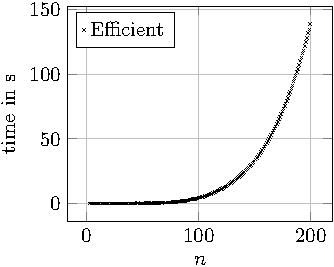
\includegraphics[scale=1]{graphic.pdf}
\caption{Execution time of algorithm \ref{alg:Efficient} for $G=[ \left\lfloor \frac{n(n+1)}{4}+1 \right\rfloor ;n,n-1,\dots,1]$ at different $n$.}
\label{fig:1234Spiel}
\end{figure}

\section{Conclusions}
For the case of weighted majority games a computational method was proposed that computes the Johnston index for all players. The time complexity and memory space complexity is bounded by $\mathcal{O}(n^3q)$ and $\mathcal{O}(nq)$ respectively.
Some examples were discussed regarding the performance.
With this method at hand practical applications of the Johnston index can be easier in the future.


\section*{References}

\bibliography{mybibfile}

\appendix

\section*{Appendix}
\begin{Pseudo-Code}
\label{alg:Efficient}
\textsl{Input: $[q;w_1,w_2,\dots,w_n]$ with $w_1\geq w_2\geq\dots\geq w_n$. }
\begin{lstlisting}[style=Pseudo-Code, mathescape=true,basicstyle=\small]
Calculate $c$
For $(i,y)\in\{1,2,\dots,n+1\}\times\{0,1,\dots,q-1\}$ set $c(i,y):=0$
$c(n+1,0):=1$
For $i = n,n-1,\dots,3$
    For $y=0,1,\dots,  \min\{w(\overline{P}_i), q-1\}$
        If $y\geq w_i$
           $c(i,y) := c(i+1,y) + c(i+1,y-w_i)$
        Else
           $c(i,y):=c(i+1,y)$
        End If
    End For
End For
Calculate $d$
For $i =n+1, n,\dots,3$
    $d(i,0):=c(i,0)$
    For $y=1,2,\dots,\min\{w(\overline{P}_i), q-1\}$
        $d(i,y):=d(i,y-1)+c(i,y)$
    End For
End For
Calculate $h$
For $y=q,q+1,\dots, \min\{q+w_n-1, w(N)\}$
    $h(n,y):=1$
End For
For $i =n-1,n-2,\dots,1$
    For $y = w_i,w_i+1,\dots,\min\{q + w_i - 1, w(P_i)\}$
        If $q + w_i - 1 - y \geq 0 \geq q - y$
           $h(i,y):=1$
        End If 
        For $j=i+1,i+2,\dots,n$
            $y_0:=\max\{0,q-y\}-1$
            $y_0:=\min\{y_0,w(\overline{P}_{j+1})\}$
            $y_1:=\min\{q+w_i-w_j-1-y, w(\overline{P}_{j+1})\}$
            If $y_1>y_0$
               $h(i,y):=h(i,y) + d(j+1,y_1)- d(j+1,y_0)$
            End If
        End For       
    End For
End For
Calculate all $\gamma_j$
For $j=1,2,\dots,n$
    $\gamma_j:=0$ 
    For $(k,y)\in\{0,1,\dots,n\}\times\{0,1,\dots,q-1\}$ set $f(k,y):=0, f_j(k,y):=0$
    For $i=1,2,\dots,n$
        Calculate $f(i-1,\cdot,\cdot)$, $f_j(i-1,\cdot,\cdot)$
        If $i=1$
           $f(0,0):=1, f_j(0,0):=1$
        Else
           For $k=i-1,i-2,\dots,1$
               For $y=q-1, q-2,\dots,w_{i-1}$
                   $f(k,y):=f(k,y)+f(k-1,y-w_{i-1})$
                   If $i-1 \neq j$
                      $f_j(k,y):=f_j(k,y)+f_j(k-1,y-w_{i-1})$
                   End If
               End For
           End For
        End If
        Update $\gamma_j$
        If $j\leq i \leq n$
            For $k=|\{p_i,p_j\}|,\dots,i$
                For $y= w(\{p_i,p_j\}),\dots, \min\{q+w_i-1,w(P_i)\}$
                    If $h(i,y)>0$
                       $f\sub{val}:=f(k-1,y-w_i)$
                       If $i>j$ And $y\leq w(P_i\setminus\{p_j\})$
                          $f\sub{val}:=f\sub{val}-f_j(k-1,y-w_i)$
                       End If
                       $\gamma_j := \gamma_j +\frac{1}{k} f\sub{val}\cdot h(i,y)$    
                    End If               
                End For
            End For
        End If
    End For 
End For
For $i=1,2,\dots,n$
    $\gamma_j:=\gamma_j/|W_\text{qmin}|$
End For
\end{lstlisting}
\textsl{Output: $\gamma_1\gamma_2,\dots,\gamma_n$. }
\end{Pseudo-Code}
The last step can be done by simply normalizing the indices or one can also use the identity
\begin{align*}
    |W_\text{qmin}|
    &=
    \sum_{i=1}^n (d(i+1,q-1)-d(i+1,q-w_i-1))
    ,
  \end{align*}
which is only valid for sorted weights $w_1\geq w_2\geq\dots\geq w_n$ and is also useful for validation purposes. Note that we need to calculate $c$ and $d$ down to $i=1$ for this.

The algorithm is very basic. For instance, obviously one do not need to calculate $\gamma_i$ for $i>1$ if $w_i=w_{i-1}$.

\end{document}